\documentclass[course=eragp]{aspdoc}

\usepackage{xstring}
\usepackage{catchfile}
\usepackage{amsmath}
\usepackage{amsfonts}
\usepackage{amssymb}
\usepackage{graphicx}
\usepackage{booktabs}
\usepackage{icomma}
\usepackage{siunitx}
\usepackage{multicol}
\usepackage{verbatim}
\usepackage{url}
\usepackage{caption}
\usepackage{subcaption}
\usepackage[german]{varioref}
\usepackage[toc]{appendix}
\usepackage{tikz}
\usepackage{pgfplots}
\usepackage{pgfplotstable}

\author{Noah Dormann \and Simon Kammermeier \and Johannes Pfannschmidt \and Florian Schmidt}
\date{Summer term 2020}
\title{Dynamic Binary Translation for RISC--V code on x86--64}

% ======= NOTE =======
% Checkout todos (--> remove before flight).
% Many unresolved issues/missing details/pending layout
% are marked by todos. Be sure to resolve all prior to
% submission.
% Hint fixes for the layout when the text is finalised.
% Until then, the floats may float.
% ====================
% --> Caro/Anna at <4568ee2160e9eac31941835333653f5d3ea033a3>
% ====================

% typeset current git commit id for drafts
% todo remove commit id before submission
\CatchFileDef{\headfull}{../../.git/HEAD}{}
\StrGobbleRight{\headfull}{1}[\head]
\StrBehind[2]{\head}{/}[\branch]
\CatchFileDef{\commit}{../../.git/refs/heads/\branch}{}
\cfoot{Draft after commit \commit on branch \branch.}

%todo name check all other usages of 'our translator' and such, maybe use a bit of variety by manually replacing the command usages.
\newcommand{\translatorname}{"INSERT PROGRAM NAME HERE"}

% define utilities and symbols
\newcommand*\diff{\mathop{}\!\mathrm{d}}
\newcommand*\Diff[1]{\mathop{}\!\mathrm{d^#1}}
\newcommand{\define}[2]{\item \textbf{#1}\\#2}
\newcommand{\conclude}[0]{\ensuremath{\Longrightarrow} }
\newcommand{\refer}[0]{\ensuremath{\rightarrow} }
\sisetup{range-phrase=--,range-units=single}
\MakeOuterQuote{"}

% list sections and subsections in toc, ignore smaller
\setcounter{tocdepth}{2}

% itemize without parskip and itemsep for compact listings
% New commands to fix editor highlighting
\newcommand{\lesslengthsep}{\setlength{\itemsep}{0ex}}
\newcommand{\lesslengthskip}{\setlength{\parskip}{0ex}}
\newenvironment{itemize*}%
  {\begin{itemize}%
    \lesslengthsep%
    \lesslengthskip}%
  {\end{itemize}}
  \newenvironment{enumerate*}%
  {\begin{enumerate}%
    \lesslengthsep%
    \lesslengthskip}%
  {\end{enumerate}}

% environment setup for pgfplots and tikz
\pgfplotsset{compat=newest}
\definecolor{era-qemu}{HTML}{FFB74D}
\definecolor{era-dbt-1}{HTML}{f44336}
\definecolor{era-dbt-2}{HTML}{64B5F6}
\definecolor{era-native}{HTML}{AED581}
\definecolor{era-dbt-3}{HTML}{ba00e5}

\begin{document}
\maketitle
\tableofcontents
\pagebreak

% \input separate files for every section! --> avoids merge conflicts

% todo @Simon replace in path for:
% don't --> do not
% hasn't --> has not
% can't --> cannot
% can not --> cannot
% todo find in path for "'s", "s'", ... @all
% todo regex for : followed by capital @all

\section{Introduction}
RISC-V is an open ISA first conceptualised in 2010 with the initial goals of research and education in mind.
In contrast to Intel's x86~\cite{intel2017man} it employs the RISC (Reduced Instruction Set Computer) scheme by providing fewer and less powerful instructions, addressing modes and cycle-heavy features in favour of a simplified micro architecture.
Its development takes the lessons learned in terms of backwards compatibility and future-proofing from other widespread ISAs like x86 into account, and aims to provide an open interface for the architecture, rather than strict implementation details.
This grants a large freedom to the implementors and greatly increases the flexibility and ease of working with the architecture~\cite[S. 1f]{riscvspec}.
As such, it looks to be open to future extensions by already defining a basis for future 128-bit integer instructions and instruction length encodings of up to 176 bits (22 bytes).
The possibility to expand further when widespread technology developments would require such an expansion is also remained open.


\subsection{Problem description}
There is already some hardware available for RISC-V\footnote{The biggest name here is probably SIFive~\cite{sifive}, which already produce multi-core CPUs with super scalar out-of-order pipelines reaching multi-GHz clock speeds.}, but it is not yet widespread.
Developers usually don't have access to real hardware, so they must instead rely on emulation to test their code written for the RISC-V platform.

\paragraph{Modes of binary translation}
When attempting to execute programs compiled for a foreign architecture on a different native one, there are essentially three distinct approaches at one's disposal.

The main principles to achieve this are:
\begin{itemize}
    \item \textbf{Interpretation}, where, much alike interpreted programming languages (e.g.\ JavaScript, Python, or Ruby), the assembly instructions located in the binary are examined while emulating the execution of the program, and equivalent actions are taken on the native system in order to simulate the guest ISA\@.
        \subitem While likely being the easiest to actually be implemented, this comes with a significant performance penalty mainly because every single assembly instruction will have to be interpreted for every execution of that program part, potentially causing a lot of redundant work.
    \item \textbf{Static Binary Translation}, where the executable is statically reverse-engineered and translated to the other architecture as a whole.
    After this translation step, it can be executed as if it were a native binary, without the need for any further special treatment.
    In theory you could reach near native speeds for the generated binary using this technique.
    There some hurdles with this though, one example is register indirect branches, which require some way to convert the foreign addresses to native at runtime.
    Any program that produces or edits assembly at runtime would also generally prove difficult to translate statically.
    \item \textbf{Dynamic Binary Translation} (DBT), which serves as a middle ground between interpreting and statically translating the executable.
    It aims to translate the program on the fly, while only focussing on the parts that are actually needed for execution.
    Therefore, it can save some of the overhead of a static translator by not spending execution time on unused code paths.
    The other aforementioned issues are also fairly easily resolved.
    Unlike an interpreter, every instruction only has to be translated once and can then be run without any unnecessary overhead.
    Of course, this assumes that the translation routines are relatively swift in performing their functions, so as not to introduce any more overhead than necessary~\cite[S. 1f.]{bintrans}.
\end{itemize}

\subsection{Motivation}
One of the most popular software emulators in general is QEMU~\cite{bellard2005qemu}\@.
While QEMU is a portable DBT that supports a wide variety of architectural combinations and ISAs, this also makes it hard to optimise it for a specific guest/host combination and therefore the program execution will be slower than necessary.

% todo User space emulation
Our aim is to provide a faster emulator, allowing the execution of RISC-V code on an x86-64 machine by means of dynamic binary translation.

The rest of this paper is structured as follows:
Section \ref{sec:Background} will define concepts and constraints relevant for our undertaking, after which section \ref{sec:Approach} will show our approach and describe the rationale for major design decisions taken during the implementation.
Select parts of the translator will then further be elaborated on in section \ref{sec:Implementation}.
Finally, sections \ref{sec:ResultsPerf} and \ref{sec:Summary} will evaluate the success and quality of our developed solutions by using standardised benchmark suites, as well as provide a short summary and future perspective of the project at hand.
















\section{Background}
\label{sec:Background}
%! Author = simon
%! Date = 22.10.20
In the following, the term \textit{host} will refer to the system of the native architecture the binary translator is built for (in our case, x86-64), and the term \textit{guest} will designate the foreign system we are attempting to emulate (RISC--V).

\subsection{Comparison of the RISC-V and x86-64 ISAs}
\label{sec:isa-cmp}
%todo (mention pseudoinstructions for later)
It is obvious that there are major differences in the two architectures, implied by RISC-V being a reduced instruction set computer (RISC) architecture and x86-64 a complex instruction set computer (CISC) architecture.

The most relevant distinction between RISC-V and x86-64 for the development of this DBT is the different address format and mismatch of general purpose and floating point registers in number.

RISC-V's load-store architecture with a three-operand instruction format allows for a better reuse of data but more instructions due to the explicit load/store operations.

x86-64 however has a register-memory architecture with a two-operand instruction format leading to more implicit/fused memory accesses being used in optimized code.

Also the very nature of translating a RISC architecture into a CISC architecture might seem like it would lead to less instructions.
In praxis the efficient fusion of multiple RISC-V instructions into single x86-64 instructions is difficult considering the fact that we are only presented with the assembly.
Even more a naive implementation leads to an instruction overhead due to the mismatch in supported operands per instruction.

Those challenges will be further elaborated on in section~\ref{sec:Approach}.

\subsection{Environment setup and memory layout}
\label{sec:memory-layout}
As the DBT is responsible for managing the execution environment of the guest binary in the shared address space, it must also handle the setup of said environment.

The header of the ELF-file (\textit{Executable and Linkable Format}) specifies which section(s) of the program need to be loaded, and where in memory they must reside.
The DBT must take care to map the file into memory correctly, while not compromising its own memory region.

Furthermore, the guest registers (see section~\vref{sec:context-switch-reg-handle}) and stack must be initialised in accordance with the architecture specification and calling convention, which necessitates a specific layout of environment and auxiliary parameters as well as command line arguments to be present~\cite[S. 2]{bintrans}.

The stack is set up exactly like the linux kernel would.
As such the stack pointer needs to point at the argument count and then towards higher addresses in order there are the zero terminated argument, environment and auxiliary vector.
Finally some alignment bytes need to be added, so the stack pointer is ABI-conformant 16 Byte aligned.
All of the information is basically just copied from the host in our case.

The memory is laid out as follows:
\begin{table}[h]
	\centering
	\begin{tabular}{rl}
		\toprule
		\textbf{Address range} & \textbf{Usage}\\
		\midrule
		0x780000000000+ & Translator address region\\
		0x77ff81000000+ & JIT generated code\\
		0x77ff807fe000+ & guest stack\\
		(last mapped address + 1)+ & guest heap\\
		defined by ELF file & mapped guest binary\\
		\bottomrule
	\end{tabular}
	\caption[Memory layout]%
	{The layout of the memory space.}
	\label{tab:}
\end{table}



\section{Approach}
\label{sec:Approach}
\subsection{Partitioning the input code}
Logically, upon facing the task of translation, the DBT must somehow divide the code into chunks it can then process for translation and execution.
The natural choice here is for the translator to partition the code into basic blocks.

Basic blocks, by definition, have only a single point of entry and exit;
all other instructions in a single block are executed sequentially and in the order that they appear in the code.
(Of course, this does not take into account mechanisms such as out-of-order execution or system calls as well as interrupt- and exception handling).

So, for our purposes, a basic block will be terminated by any control-flow altering instruction like a jump, call or return statement, or a system call\footnote{These may or may not have control-flow altering effects; they in any case need to be handled this way due to the reasons laid out in section~\vref{sec:syscall-handling}.}.

% todo continued about basic blocks, jump/call instructions, etc.


\subsection{Translating the partitioned code}
The most basic idea for translating the now partitioned basic blocks is to have a fixed association that maps every instruction in the guest ISA to a sequence of instructions native to the host.

The quality of the code that can be easily generated here strongly depends on the properties of the host and guest architectures in question.
Difficulties can arise due to differences in the instruction operand formats and the type of instruction set architecture the DBT is dealing with.

In our case, as outlined in section~\vref{sec:isa-cmp}, challenges stem from the fact that we are translating code from a load-store architecture using a three-operand instruction format into a register-memory architecture in which (generally) one of the source operands is also the implicit destination operand.
This, for example, means that a single arithmetic \texttt{add rd, rs1, rs2} in RISC-V assembly language generally can not be translated via a single instruction, but rather requires two instructions: moving \texttt{rs1} to \texttt{rd}, then adding the value of \texttt{rs2} to \texttt{rd}.

Opportunities for optimisation lie wherever there is a way to shorten the translation's amount of CPU clock cycles, possibly by employing semantically equivalent native instructions that run in a shorter timespan.
The RISC-V pseudoinstructions (as mentioned in section~\ref{sec:isa-cmp}) are also of some help here~\cite[S. 139]{riscvspec}, as it is clear that an instruction like \texttt{xori x10, x10, -1} can be directly translated as a \texttt{not x10}, without needing to resort to \texttt{mov} and \texttt{xor}.


\subsection{Code cache and block handling}
Naturally, the DBT aims to store the translated code in a semi-permanent way, for it is the goal to not have to translate a required section more than once.

For that, we allocate a region of memory reserved for the basic block translations, also called a \textit{code cache}.
Additionally, an index to this memory section is required, since there needs to be a way to quickly reference the blocks residing in the cache and associate them with both the host and guest instruction pointers that identify them during execution.

% todo info about chaining and optimisations

It is possible that this code cache might fill up during the execution of a large guest program.
If it does, there are two different strategies to handle this issue:
One can either invalidate and purge some or all of the blocks currently residing in the cache, or dynamically resize the cache according to the needs of the guest program~\cite[S. 3]{bintrans}.

Purging the entire cache would require the translator to restart translation on older blocks that might be needed again, introducing a performance overhead that needs to be weighed against the higher memory usage of enlarging the cache.

On the other hand, selective deletion of some of the blocks in the cache is very difficult due to optimisations taken in the context of chaining.
As any chained jumps located in another cached block are dependent on the target block residing in the cache, the target's removal would invalidate these jumps.
It would thus only be possible to either remove all blocks with jump references to the candidate up for removal, or to leave all blocks with jump references in the cache altogether.


\subsection{Register handling and context switching}
\label{sec:context-switch-reg-handle}
As outlined in section~\ref{sec:isa-cmp}, the RISC-V and x86-64 architectures have differing amounts of general purpose registers.
In some way, the state of the 32 general purpose registers \texttt{x1}\footnote{\texttt{x0} is hardwired to a constant zero. All reads will return 0, all writes will be ignored. Hence, this register needs special handling in the DBT.} to \texttt{x31} and the \texttt{pc} needs to be stored and available to the translations of the identified basic blocks.

As x86-64 only provides for 16 general-purpose registers (\texttt{rax--rdx, rsi, rdi, rsp, rbp and r8--r15}), it is impossible to directly and statically map all guest registers to native host registers.
Adding to the above, due to the fact that some x86-64 registers have special or implicit purposes in some instructions (\texttt{rax} and \texttt{rdx} in \texttt{(i)mul}, \texttt{cl} in shifting, etc.), care must be taken in choosing the registers that can be used for such a mapping.
Keeping a guest register file exclusively in memory, and loading them into native registers when needed within the translations of single instructions is technically possible, especially in light of x86-64's ability to extensively use memory operands in the instructions.
However, this necessitates a large number of memory accesses for both memory operands in the instructions as well as local register allocation within the translated blocks.
Due to the very large performance gain connected to using register operands instead of memory operands, this is also not feasible at scale~\cite[S. 8f.]{bintrans}.

Accordingly, the solution would be an approach that employs parts of both of these extremes~\cite[S. 9]{bintrans}.
We aim to employ the tools we design to discover the most-used registers in the guest programs, and statically map these to general purpose x86-64 registers.
The remaining operands can either be used from memory directly, or dynamically allocated into free host registers inside a single block's translation.
Thus, we save much overhead otherwise spent on memory access to the register file, but do not unnecessarily occupy native register space with seldomly accessed guest registers.

% todo context switching




\subsection{System call handling}
\label{sec:syscall-handling}
System calls are also a very important part of enabling the guest program's execution.
Thus, every ISA must offer some way to switch the execution context in the kernel mode for the system call to be handled.

For RISC-V, the instruction \texttt{ECALL} (for \textit{environment call}, formerly \texttt{SCALL}) handles these requests, with the system call number residing in register \texttt{a7} and the arguments being passed in \texttt{a0--a6}.

However, the DBT generally cannot just reorganise the guest argument values and system call identifier according the host's calling convention and relay the system call directly.
The RISC-V guest program expects a different operating system kernel than is present natively on the host;
with that, the system call interface also differs~\cite[S. 2f.]{bintrans}.

In order to handle the \texttt{ECALL} instruction correctly, the translator must thus build the translated instruction to call a specific handler routine not too dissimilar from one that may be found in a kernel.
There, system calls that exist natively on the host architecture as well (like \texttt{write} or \texttt{clock\_gettime}) can usually be passed along to the host's kernel directly.

Care must be taken for system calls that would enable the guest to change the state or context of the host -- an \texttt{mmap} into the translator's memory region, for example, or a call to \texttt{exit} -- these calls must be emulated accordingly to prevent these faults.
In cases where the data structure layout used by the kernels differs, the DBT must also perform necessary actions to adapt the formats to each other.
Some system calls may not exist at all on the native architecture of the host, it is up to the DBT to emulate the required functionality~\cite[S. 2f.]{bintrans}.




















\section{Implementation Details}
\label{sec:Implementation}
The following section aims to provide an in-depth overview of the system's architecture as well as the rationale for major design decisions taken during the implementation.

\subsection{System architecture and execution control flow}
% todo overview, add class diagrams and flow charts

\subsection{Instruction translation process}
% todo add reference to faenc
The decoding of the RISC-V assembly is quite straight forward as we have a fixed instruction length of 32bit.
Thus, the assembly is parsed in 4byte blocks with the information beeing extracted in an intermediate instruction format, holding the instruction mnemonic, operands and immediates in uncompressed form.
This intermediate format can then be used by special per mnemonic translation functions which in the end generate the x86-64 byte code using faenc.

\subsection{Code cache and TLB for block lookup}
% todo

\subsection{Static hybrid register mapping}
\subsubsection{Register priority analysis}
In order to achieve the best performance with the hybrid approach to the register mapping described in section~\vref{sec:context-switch-reg-handle}, we must decide which registers of the RISC-V guest to map into the host's limited number of available GPRs.
There are two main ways of determining the priority of registers when considering them as candidates for a mapping.

It is, on the one hand, possible to assess the priority statically, by performing an analysis of the binary in question.
Essentially, the hereby produced metric counts the number of times the register is used in the assembly instructions listed in the guest program and thus delivers an idea of how important each register is to this specific executable.
We have built the tools required for this effort directly into the translator's analyser function, accessed via the \texttt{-a} flag.

However, this approach does not take into account that a single instruction may be executed many times while the program is running.
Accordingly, the other approach is to assess the register priority dynamically by analysing and profiling the execution of the testing program, thereby gaining an insight into how often each register is actually used during the execution.
The translator is also capable of performing such an analysis, commanded by the \texttt{-p} flag.
A dynamic analysis, of course, delivers a largely more accurate idea of the priority of the registers in question, but has the decided and obvious disadvantage that it cannot be performed without actually executing the binary.


% todo plot goes here


% todo add ref
For the average results of such an analysis performed on a range of programs, including \textit{gzip}~\cite{gzip} and several benchmarks of the \texttt{intspeed}-Suite of \textit{SPEC CPU 2017}~\cite{spec-cpu-2017}, see figure~NUMBERGOESHERE.

Primarily, we gain interesting insights into the differences between the static and dynamic results yielded by the analysis.
While the static ranked hit list does not differ greatly between the different executables and the top $12$ entries are identical for every one of the tested programs, the dynamic results are far more variable.
This makes creating a register mapping that fits well to every executable very difficult.

The benchmarks \texttt{605.mcf\_s} (route planning workload) and \texttt{620.omnetpp\_s} (discrete event simulation for computer networking)~\cite{spec-cpu-doc} of the \textit{SPEC CPU} suite can serve as examples here.
For programs like \texttt{605.mcf\_s} that only lightly use the stack, holding the stack pointer \texttt{sp/x2} in a native register when only $1,20\,\%$ of accesses actually utilise it would not be necessary.
However, other programs like \texttt{620.omnetpp\_s} may rely heavily on the stack, and thus log very frequent accesses to \texttt{sp/x2};
when statistically every ninth access is to the stack pointer, it is absolutely essential to map the register to a native GPR\@.

If a static analysis yielded results of similar quality to the dynamic counterpart, the DBT could analyse the binary prior to execution and run every program with a best-fit static register mapping.
However, evidently, this is impossible with dynamic profiling.


\subsubsection{Structure of the mapping}
When we structure our mapping by the average case of the insights gained, we statistically capture about $83,59\,\%$ of register accesses, initially leaving the remaining $16,41\,\%$ to read from the register file in memory.

From the 16 general-purpose registers x86-64 has to offer, we may use the 12 registers \texttt{rbx}, \texttt{rbp}, \texttt{rsi}, \texttt{rdi} and \texttt{r8}--\texttt{r15}.
The remaining registers have either implicit or exclusive functions in some instructions (\texttt{rax} and \texttt{rdx} for multiplication/division, \texttt{cl} for shifting), or, like \texttt{rsp}, are impractical to use in combination with block chaining and function calls.

Taking the 12 registers that are most accessed on average, the mapping structure is as seen in table~\vref{tab:static-register-mapping}.

\begin{table}
	\centering
	\begin{tabular}{rcccccccccccc}
		\toprule
		\textbf{RISC-V register} & \texttt{a5} & \texttt{a4} & \texttt{a3} & \texttt{a0} & \texttt{fp} & \texttt{sp} & \texttt{a2} & \texttt{a1} & \texttt{s1} & \texttt{ra} & \texttt{a7} & \texttt{s2}\\
		\textbf{x86-64 mapping} & \texttt{rbx} & \texttt{rbp} & \texttt{rsi} & \texttt{rdi} & \texttt{r8} & \texttt{r9} & \texttt{r10} & \texttt{r11} & \texttt{r12} & \texttt{r13} & \texttt{r14} & \texttt{r15}\\
		\bottomrule
	\end{tabular}
	\caption[Active static register mapping]%
	{The static register mapping in use by the translator, ordered by the RISC--V register usage frequency (descending).}
	\label{tab:static-register-mapping}
\end{table}

\subsubsection{Dynamically allocated replacement registers}
% todo details about the lazy_replace mapping
In order to implement the desired temporary register replacement behaviour detailed in section~\ref{sec:context-switch-reg-handle}, we need to keep track of the age of the values currently situated in the replacement registers.
To do this, we track a metric of \textit{replacement recency} (essentially serving as an inverse value age) for each block during translate-time.
This recency gets incremented for every access not captured by the static register mapping.

An access to a register that is not statically mapped then first checks the contents of all temporary registers -- if the value is already present, the DBT may use that value's register.
If it is not already present, the DBT selects any free replacement register if able, and otherwise selects the register with the oldest value (or minimal recency) for write-back.
The value is then loaded into the selected register from the register file in memory and marked as being the youngest in order to prevent it from being discarded in following mapping calls.

The dynamic mapping must also be able to receive requests for specific target registers for a load in order to support shifting and multiplication/division instructions that require arguments in implicitly defined registers.
In order to support this efficiently, the DBT is able to shuffle the values in the replacement registers around accordingly.

With this behaviour, we manage to greatly save on memory accesses to the register file compared to simply loading and storing the values on an instruction-by-instruction basis.
This style of register mapping can also not perform worse than accessing memory for each instruction, as in the worst case the DBT will perform the same memory accesses as with the other strategy, just possibly at a different time.


\subsection{Context switching details}
% todo context switching

\subsection{Optimisation of the generated code}
\label{sec:optimise}
\subsubsection{Block chaining}
\subsubsection{Recursive jump translation}
\subsubsection{Return address stack}
\subsubsection{Macro operation fusion by pattern matching}
% todo optimisation details, maybe split up? more sections?

\subsection{Detailed system call overview}
% todo special description for emulated calls

As described in section~\vref{sec:syscall-handling}, we must assume the role of the kernel by handling system calls during the execution of the guest program.
We achieve this by translating the \texttt{ECALL} instruction as a context switch and jump to the \texttt{emulate\_ecall} routine in the DBT, which can then take the appropriate action.

As we stored the guest's registers before jumping to the handler, the requested system call index is now available to the DBT in the register file as entry \texttt{a7}, as per the RISC-V standard calling convention.
We may now handle the system calls based on that index and the arguments passed in the registers \texttt{a0} through \texttt{a6}, and write the return value to entry \texttt{a0} of the register file prior to switching the context back to the guest.

As previously mentioned, some system calls require special handling when encountered by the DBT (see table~\vref{tab:syscall-special} for details).
The following will describe the specifics of these issues with system calls that are either not present on the x86-64 host architecture, or may influence or break the state of the DBT\@.
\begin{description}
	\item[Adapting structure data format.]
	There are system calls like \texttt{fstat} and \texttt{fstatat} that exist both on RISC-V as well as x86-64, but use different data structure layouts in their return values.
	Thus, the DBT must adapt the host's returned data to the required format prior to passing it back to the guest.
	
	
	\item[Emulation required.]
	The DBT captures the \texttt{exit} and \texttt{exit\_group} calls.
	Passing them through would immediately terminate the DBT -- an action that is undesirable as it prevents any form of clean-up or post-execution profiling and analysis to take place.
	Thus, the DBT uses these system calls to set a flag which stops the translator's main loop from executing the next iteration.
	
	The \texttt{brk} system call must also be entirely emulated, as it would otherwise allow the guest program to modify the endpoint of the DBT's data segment (\textit{program break}), thus potentially deallocating some of the translator's memory.
	
	
	\item[Ignoring system calls.]
	% todo expand the rationale here. is this correct?
	The \texttt{rt\_sigaction} system call is ignored by the DBT, as any signals received by the process will be handled by the translator due to the fact that the guest program's execution is emulated in the DBT's process.
	
	
	\item[Guarded pass-through to host.]
	Essentially, any system call that has the possibility to influence the state or memory of the translator needs to have respective safe-guards in place.
	A good example of this behaviour is the \texttt{mmap} system call, the handling of which also reflects the memory layout scheme discussed in section~\vref{sec:memory-layout}.
	
	In any case, we must prevent a memory mapping into the translator's memory region.
	Mappings that do not interfere with the DBT's memory can be passed along to the host directly.
	In case a hinted mapping would conflict with the translator's memory, we may just re-hint the mapping to the top of the guest's address space.
	When the call is not hinted (the \texttt{MAP\_FIXED} or \texttt{MAP\_FIXED\_NOREPLACE} flag commands the mapping at exactly the specified address), we are unable to provide the guest with the requested mapping;
	thus we simulate an existing mapping in the location in question by returning \texttt{EEXIST} for \texttt{MAP\_FIXED\_NOREPLACE} and failing the call with \texttt{EINVAL} for \texttt{MAP\_FIXED}.
	
	Similarly, we fail the guest's \texttt{munmap} with \texttt{EINVAL} in cases where the translator's memory would be compromised by the deallocation.
\end{description}

The other supported system calls may be directly passed through to the host after performing the necessary index mapping.
With this strategy, we are able to support the following system calls:
\begin{multicols}{4}
	\begin{itemize*}
		\item \texttt{getcwd}
		\item \texttt{fcntl}
		\item \texttt{ioctl}
		\item \texttt{unlinkat}
		\item \texttt{ftruncate}
		\item \texttt{faccessat}
		\item \texttt{chdir}
		\item \texttt{fchmod}
		\item \texttt{fchown}
		\item \texttt{pipe2}
		\item \texttt{openat}
		\item \texttt{close}
		\item \texttt{getdents64}
		\item \texttt{lseek}
		\item \texttt{read}
		\item \texttt{write}
		\item \texttt{writev}
		\item \texttt{readlinkat}
		\item \texttt{utimensat}
		\item \texttt{set\_tid\_address}
		\item \texttt{futex}
		\item \texttt{set\_robust\_list}
		\item \texttt{clock\_gettime}
		\item \texttt{tgkill}
		\item \texttt{rt\_sigprocmask}
		\item \texttt{uname}
		\item \texttt{gettimeofday}
		\item \texttt{getpid}
		\item \texttt{getuid}
		\item \texttt{geteuid}
		\item \texttt{getgid}
		\item \texttt{getegid}
		\item \texttt{gettid}
		\item \texttt{sysinfo}
		\item \texttt{execve}
		\item \texttt{wait4}
		\item \texttt{prlimit64}
		\item \texttt{renameat2}
		\item \texttt{getrandom}
	\end{itemize*}
\end{multicols}

\begin{table}
	\centering
	\begin{tabular}{ccc}
		\toprule
		\textbf{System Call (index)} & \textbf{Handling} & \textbf{x86-64 base (index)}\\ 
		\midrule
		\texttt{fstatat} (79) & data reformat & \texttt{newfstatat} (262)\\
		\texttt{fstat} (80) & data reformat & \texttt{fstat} (5)\\
		\texttt{exit} (93) & emulate & n/a\\
		\texttt{exit\_group} (94) & emulate & n/a\\
		\texttt{rt\_sigaction} (134) & ignore & n/a\\
		\texttt{brk} (214) & emulate & n/a\\
		\texttt{munmap} (215) & guarded pass-through & \texttt{munmap} (11)\\
		\texttt{mmap} (222) & guarded pass-through & \texttt{mmap} (9)\\
		\bottomrule
	\end{tabular}
	% todo keep up-to-date
	% state: aa55cef4816eb790df21f4742b7cf1f29685da49
	\caption[Specially handled system calls overview]%
	{An overview of the system calls we support that require special handling by the binary translator.}
	\label{tab:syscall-special}
\end{table}






\section{Results and Performance}
\label{sec:ResultsPerf}
The following section will give an overview of the methods used to test the programs correctness and performance, as well as lay out the results of these tests.
\subsection{Verification}
The correctness of our translator is checked by extensive unit tests, which are used to check if the translations of a the RISC--V instruction perform the operations that are expected as per the architecture specification.

Using the parameterised tests provided by the Google~Test~\cite{gtest} framework, we are able to test a variety of different input values and combinations of statically mapped or not mapped register operands.
Different combinations of using the same register and zero register \texttt{x0} for in- and output are also tested.
Apart from this, correctness is also confirmed by being able to successfully run the \textit{SPEC CPU 2017} benchmark suite as described in section~\ref{subsec:spec-cpu-2017-benchmark-suite} below.


\subsection{SPEC CPU 2017 Benchmark Suite}
\label{subsec:spec-cpu-2017-benchmark-suite}


\begin{table}
	\centering
	\begin{tabular}{rl}
		\toprule
		\textbf{SPECspeed Benchmark} & \textbf{Workload}\\
		\midrule
		\texttt{600.perlbench} & Perl interpreter\\
		\texttt{602.gcc} & GNU C compiler\\
		\texttt{605.mcf} & Route planning\\
		\texttt{620.omnetpp} & Discrete Event simulation -- computer network\\
		\texttt{623.xalancbmk} & XML to HTML conversion via XSLT\\
		\texttt{625.x264} & Video compression\\
		\texttt{631.deepsjeng} & Artificial Intelligence: alpha-beta tree search (Chess)\\
		\texttt{641.leela} & Artificial Intelligence: Monte Carlo tree search (Go)\\
		\texttt{648.exchange2} & Artificial Intelligence: recursive solution generator (Sudoku)\\
		\texttt{657.xz} & General data compression\\
		\bottomrule
	\end{tabular}
	\caption[SPEC CPU 2017 workload description]%
	{A description of the workloads covered by the \textit{SPEC CPU 2017} \texttt{intspeed} suite~\cite{spec-cpu-doc}.}
	\label{tab:spec-description}
\end{table}


Measuring the performance of the DBT was accomplished by using the tools in \textit{SPEC CPU 2017} \texttt{intspeed} suite of benchmarks.
This not only generates reproducible and widely accepted results in the industry, it also validates the results produced during the run, thus ruling out any errors in the translations of the benchmarks.

The \texttt{intspeed} suite also presents a variety of different workloads to the translator that are based on real-life scenarios, thus producing an accurate and understandable overview of the performance in a non-controlled environment. % name
An overview of the workloads covered by the aforementioned suite can be found in table~\ref{tab:spec-description}.
Further context is provided by performance testing using the data compression utility \textit{gzip}~\cite{gzip}, where compression time is compared between runs on a native machine, in QEMU and in the DBT\@.

All testing was performed on an x86--64 8-core \textit{Intel Xeon Bronze 3106} system clocked at $1,70$ GHz base with $78$ GiB of physical memory, running \textit{Ubuntu 18.04.3 LTS}, kernel version \textit{4.15.0-70-generic}.
The DBT was compiled via \texttt{CMAKE\_BUILD\_TYPE} set to \texttt{Release} and \texttt{CMAKE\_INTERPROCEDURAL\_OPTIMIZATION} enabled, which implies \texttt{-O3} and \texttt{-flto -fno-fat-lto-objects}.

The benchmarks were compiled using compiler optimisation level \texttt{-O3} and linked statically.
For the native run, \texttt{-march=x86-64} was used on GCC version 7.5.0 from the default Ubuntu package repository.
The RISC--V binaries for our translator and QEMU were compiled using \texttt{-march=rv64ima} and \texttt{-mabi=lp64}.
For this, a self-compiled GCC with the sources taken from the official toolchain repository at version 10.1.0 was used.
This made it necessary to also specify \texttt{-fcommon -fallow-argument-mismatch} to stay fully compatible.

\subsubsection{Results}
Figure~\vref{fig:spec-results} shows normalized performance results of the \textit{SPEC CPU 2017} \texttt{intspeed} benchmarks, effectively showing how much overhead QEMU and our translator caused versus the same benchmark compiled and run natively.
Some of the overhead must of course be attributed to the architectural differences between x86 and RISC--V resulting in needing more instructions in RISC-V assembly than x86.
This means these results do not directly measure the overhead vs.\ native that the whole translator infrastructure (parsing, translation, code cache etc.) causes.
What we can compare though, is the relative results of QEMU and our translator, since both use the same compiler and thus get the same binary. % name
This means the results are a measure for the relative efficiency of the infrastructure and the quality of the generated code.

Through the various performance optimisations mentioned in section~\vref{sec:optimise}, we are able to reach our goal of consistently outperforming QEMU\@.
In some cases the advantage is only slight, but in other workloads like the 602.gcc compiler benchmark the advantage grows to a comfortable $80\,\%$.

Most benchmarks show runtimes of about $1.9$x native with \texttt{625.x264} and \texttt{600.perlbench} being the outliers.

% ======= SPEC CPU Results =======
% Results of the intspeed SPEC CPU 2017 runs.
% ================================

\newcommand{\addAvg}[3]{ %
% #1=table name
% #2=first column name
% #3=list of columns to decorate
% Transpose the table, so we can work on rows instead of columns
\pgfplotstabletranspose[colnames from={#2},input colnames to={#2}]{\intermediatetable}{#1}
\pgfplotstablecreatecol[
    create col/assign/.code={%
      \def\entry{}
      \foreach \i in {#3} {
        \ifnum\pgfplotstablerow=\i
        \def\colsum{0}
                  \pgfmathtruncatemacro\maxcolindex{\pgfplotstablecols-1}
                  \pgfplotsforeachungrouped \col in {1,...,\maxcolindex}{
                      \pgfmathsetmacro\colsum{\colsum+\thisrowno{\col}}
                  }
          \pgfmathsetmacro\colmean{\colsum/(\pgfplotstablecols-1)}
          \xdef\entry{\colmean}
        \fi
      }
      \pgfkeyslet{/pgfplots/table/create col/next content}\entry
    }
]{Avg}\intermediatetable

% Transpose back to the original form
\pgfplotstabletranspose[colnames from=#2, input colnames to=#2]{#1}{\intermediatetable}
}
%

\pgfplotstableread[col sep=comma]{benchmarks/spec-base/native.csv}\nativetable
\pgfplotstableread[col sep=comma]{benchmarks/spec-base/dbt.csv}\dbttable
\pgfplotstablecreatecol[create col/copy column from table=\nativetable{Est. Base Run Time}]{native}\dbttable
\pgfplotstablecreatecol[create col/expr={\thisrow{Est. Base Run Time} / \thisrow{native}}]{ratio}\dbttable
\addAvg{\dbttable}{Benchmark}{12}
%\pgfplotstabletypeset[
%  columns/Benchmark/.style={string type},
%  columns={Benchmark, ratio}]{\dbttable}

\begin{figure}[h]
	\centering
	\begin{tikzpicture}
		\begin{axis}[%
			title = {SPEC CPU 2017 \texttt{intspeed} Results},
			ybar,
			area legend,
			ylabel = {Execution time [ratio to native]},
			xtick = data,
			xtick style = {draw = none},
			xticklabel style = {
				inner sep = 0pt,
				anchor = north east,
				rotate = 60
			},
			ytick = {1.0, 2.0, 3.0, 4.0, 5.0, 6.0},
			scaled y ticks = false,
			xticklabels from table={\dbttable}{Benchmark},
			ymin = 0, ymax = 6.5,
			ymajorgrids = true,
			bar width = 5pt,
			height = 7.0cm,
			width = 0.9\linewidth,
			legend style = {
				at = {(0.98, 0.97)},
				anchor = north east,
				legend columns = 3,
				column sep = 0.2cm
			}
		]
			% Native results
			\pgfplotstableread[col sep=comma]{benchmarks/spec-base/native.csv}\nativelocaltable
			\pgfplotstablecreatecol[create col/copy column from table=\nativetable{Est. Base Run Time}]{native}\nativelocaltable
			\pgfplotstablecreatecol[create col/expr={\thisrow{Est. Base Run Time} / \thisrow{native}}]{ratio}\nativelocaltable
			\addAvg{\nativelocaltable}{Benchmark}{12}
			\addplot+[fill=era-native, draw=black] table [x expr=\coordindex, y=ratio] \nativelocaltable;

			% QEMU results
			\pgfplotstableread[col sep=comma]{benchmarks/spec-base/qemu.csv}\qemutable
			\pgfplotstablecreatecol[create col/copy column from table=\nativetable{Est. Base Run Time}]{native}\qemutable
			\pgfplotstablecreatecol[create col/expr={\thisrow{Est. Base Run Time} / \thisrow{native}}]{ratio}\qemutable
			\addAvg{\qemutable}{Benchmark}{12}
			\addplot+[fill=era-qemu, draw=black] table [x expr=\coordindex, y=ratio] \qemutable;

			% DBT results
			\addplot+[fill=era-dbt-1, draw=black] table [x expr=\coordindex, y=ratio] \dbttable;

			\legend{native, QEMU, DBT}
		\end{axis}
	\end{tikzpicture}
	\caption[SPEC CPU 2017 Results]%
	{Results of \texttt{ref}-workload runs of \textit{SPEC CPU 2017} \texttt{intspeed} (normalised, lower is better).}
	\label{fig:spec-results}
\end{figure}
% ================================

\subsubsection{Analysis}
% todo @Simon: Sec. 5.2.2 zu 625: Warum ist das euer DBT hier nur unwesentlich schneller als QEMU, im Vergleich zu anderen Benchmarks?
% todo @Simon: Sec. 5.2.2 zu 600: Dafuer habt ihr doch Chaining? Unklar.
% todo @Simon: Sec. 5.2.2: Fehlt: Was fehlt, um besser an die native Kompilierung heranzukommen? Warum ist euer DBT besser als QEMU? Die Antworten koennen auch nach 5.3 (oder (vielleicht besser?) in einer neuen "5.5 Discussion") gegeben werden -- aber irgendwo solltet ihr Antworten haben.

\texttt{625.x264} on x86 heavily takes advantage of vectorisation, which RISC-V does not yet support, meaning that the compiler will have to generate loops that run more often, thus needing significantly more instructions for the same result.
Retrospective vectorisation on the translator side is not easy since this would involve detecting the vectorisable loop patterns on assembler level, a task that even the compiler often isn't very effective at, even though it has the knowledge of the entire program.
There are also instances where it relies heavily on 32 bit integer arithmetic, which in RISC-V always causes the results to be sign extended to the 64 bit register width, in comparison to x86 which zero extends in these cases.
Thus many consecutive 32 bit instructions on the same values cause a lot of redundant sign extensions.
A future version of the translator could do the sign extensions lazily to save on a bunch of redundant work in some cases.

The \texttt{600.perlbench} on the other hand has a lot of conditional branches and jumps in the hot blocks.
This causes a lot of context switches since recursive translation currently is only employed for unconditional branches/calls.
Recursively translating the path that is considered hot by the compiler could improve performance by a bit.
It also potentially causes redundant work for the translator, since jumps to the middle of a basic block currently are handled by treating it like a new block beginning at the jump target.



\subsection{Evaluation of translator optimisations}
\begin{table}
	\centering
	\begin{tabular}{rl}
		\toprule
		\textbf{Option} & \textbf{Description}\\
		\midrule
		\texttt{no-ras} & Disable the return address stack\\
		\texttt{no-chain} & Disable block chaining\\
		\texttt{no-jump} & Disable recursive jump target translation\\
		\texttt{no-fusion} & Disable macro operation fusion\\
		\texttt{none} & All of the above\\
		\bottomrule
	\end{tabular}
	% state: 5afb8706e482917866a3507a54d1512befe56a21
	\caption[Translator optimisation options]%
	{The options for translator optimisations, as seen in \texttt{----optimize=help}.}
	\label{tab:opt-options}
\end{table}

In order to evaluate the optimisations built into the translator, we ran the \textit{SPEC CPU 2017} suite with various combinations of the available optimisation options in the same translator version (\texttt{v1.3.1}, the final release in the project's main development cycle).

The results of these runs can be seen in figure~\ref{fig:opt-compare}, and an overview of the specified switches can be found in table~\ref{tab:opt-options}.

% ======= Optimisation comparison results =======
% Results of the optimisation option comparisons.
% Show all SPEC run results and analyse below.
% ===============================================
\pgfplotstableread[col sep=comma]{benchmarks/spec-compare/base.csv}\basetable
\pgfplotstableread[col sep=comma]{benchmarks/spec-compare/no-ras.csv}\norastable
\pgfplotstableread[col sep=comma]{benchmarks/spec-compare/no-fusion.csv}\nofusiontable
\pgfplotstableread[col sep=comma]{benchmarks/spec-compare/no-jump-no-ras.csv}\nojumpnorastable
\pgfplotstableread[col sep=comma]{benchmarks/spec-compare/none.csv}\nonetable

\pgfplotstablecreatecol[create col/copy column from table=\basetable{Est. Base Run Time}]{base}\basetable
\pgfplotstablecreatecol[create col/expr={\thisrow{Est. Base Run Time} / \thisrow{base}}]{ratio}\basetable
\addAvg{\basetable}{Benchmark}{12}

\pgfplotstablecreatecol[create col/copy column from table=\basetable{Est. Base Run Time}]{base}\norastable
\pgfplotstablecreatecol[create col/expr={\thisrow{Est. Base Run Time} / \thisrow{base}}]{ratio}\norastable
\addAvg{\norastable}{Benchmark}{12}

\pgfplotstablecreatecol[create col/copy column from table=\basetable{Est. Base Run Time}]{base}\nofusiontable
\pgfplotstablecreatecol[create col/expr={\thisrow{Est. Base Run Time} / \thisrow{base}}]{ratio}\nofusiontable
\addAvg{\nofusiontable}{Benchmark}{12}

\pgfplotstablecreatecol[create col/copy column from table=\basetable{Est. Base Run Time}]{base}\nojumpnorastable
\pgfplotstablecreatecol[create col/expr={\thisrow{Est. Base Run Time} / \thisrow{base}}]{ratio}\nojumpnorastable
\addAvg{\nojumpnorastable}{Benchmark}{12}

\pgfplotstablecreatecol[create col/copy column from table=\basetable{Est. Base Run Time}]{base}\nonetable
\pgfplotstablecreatecol[create col/expr={\thisrow{Est. Base Run Time} / \thisrow{base}}]{ratio}\nonetable
\addAvg{\nonetable}{Benchmark}{12}

\begin{figure}[h]
	\centering
	\begin{tikzpicture}
		\begin{axis}[%
			title = {Optimisation option evaluation},
			ybar,
			area legend,
			ylabel = {Execution time [ratio to base]},
			xtick = data,
			xtick style = {draw = none},
			xticklabel style = {
				inner sep = 0pt,
				anchor = north east,
				rotate = 60
			},
			xticklabels from table={\basetable}{Benchmark},
			ytick = {0.5, 1,1.2,1.4,1.6,1.8,2.0},
			ymin = 0.5, ymax = 2,
			ymajorgrids = true,
			bar width = 3.5pt,
			height = 8.0cm,
			width = 0.95\linewidth,
			legend style = {
				at = {(0.98, 0.97)},
				anchor = north east,
				legend columns = 2,
				column sep = 0.2cm
			}
		]
			% base results
			\addplot+[fill=era-native, draw=black] table [x expr=\coordindex, y=ratio] \basetable;
			
			% no-fusion results
			\addplot+[fill=era-dbt-1, draw=black] table [x expr=\coordindex, y=ratio] \nofusiontable;

			% no-ras results
			\addplot+[fill=era-qemu, draw=black] table [x expr=\coordindex, y=ratio] \norastable;
			
			% no-jump-no-ras results
			\addplot+[fill=era-dbt-2, draw=black] table [x expr=\coordindex, y=ratio] \nojumpnorastable;
			
			\legend{base, \texttt{no-fusion}, \texttt{no-ras}, \texttt{no-jump}{,~} \texttt{no-ras}}
		\end{axis}
	\end{tikzpicture}
	\caption[Translator optimisation evaluation results]%
	{Results of \texttt{ref}-workload runs of \textit{SPEC CPU 2017}s \texttt{intspeed} with various optimisation option combinations (normalised, lower is better).}
	\label{fig:opt-compare}
\end{figure}


\pgfplotstableset{
	% define how the ’new’ column shall be filled:
	create on use/Benchmark/.style={create col/copy column from table=\basetable{Benchmark}}
}
\pgfplotstableset{% Global config
    every head row/.style={before row=\toprule,after row=\midrule},
    assign column name/.style={/pgfplots/table/column name={\textbf{#1}}},
    every last row/.style={after row=\bottomrule},
}
\pgfplotstablenew[columns={Benchmark}]{10}\printtable
\pgfplotstablecreatecol[create col/copy column from table=\norastable{ratio}]{no-ras}\printtable
\pgfplotstablecreatecol[create col/copy column from table=\nojumpnorastable{ratio}]{{no-jump, no-ras}}\printtable
\pgfplotstablecreatecol[create col/copy column from table=\nofusiontable{ratio}]{no-fusion}\printtable
\pgfplotstablecreatecol[create col/copy column from table=\nonetable{ratio}]{none}\printtable

\begin{table}[h]
\centering
\pgfplotstabletypeset[columns/Benchmark/.style={string type},/pgf/number format/fixed, /pgf/number format/precision = 2,/pgf/number format/fixed zerofill=true]{\printtable}
\caption[Optimisation results]{Optimisation results data (including \texttt{----optimize=none} run), normalised to base.}
\label{tab:table-optim}
\end{table}
% ================================


Macro operation fusion does not seem to provide a large performance benefit, in most benchmarks the numbers do not even suggest any performance increase above natural deviation of benchmark runs.
This means the implemented pattern matching does not give the desired effect of a good performance increase.
Further tweaking of the checked patterns might make this optimisation more worthwhile.

The return address stack provided for a significant advantage in some benchmarks.
Especially the function call heavy \texttt{620.omnetp}, \texttt{623.xalancbmk}, \texttt{631.deepsjeng}, \texttt{641.leela} benchmarks showed good performance gains of over $50\,\%$.
The \texttt{600.perlbench}, as well as the \texttt{648.exchange2} and \texttt{657.xz} benchmarks where most of the runtime is spent in only a couple loops naturally could not benefit a lot.

Recursive jump translation without also utilising the return address stack only provided a performance increase over disabling both in some benchmarks.
The main reason for this might be that this also makes context switches necessary on unconditional jumps that aren't function calls or returns.
This makes jump-heavy benchmarks take a performance hit while jump-light benchmarks are almost unaffected.

Expectedly, the highest performance penalty was incurred by disabling chaining as well.
This makes a context switch back to the translator necessary for every executed basic block.
The benchmarks that are less impacted by disabling block chaining are the ones where fewer basic blocks were executed relative to their runtime.
This correlates with the fact that the most executed blocks of these benchmarks contain more instructions and hence execute for a longer time.

Furthermore, the lazy replacement register handling described in section~\ref{sec:reg-handle} had a high impact in some benchmarks, most notably \texttt{657.xz}, providing for a roughly $45\,\%$ performance increase -- more than any other optimisation apart from block chaining.
Any workload that frequently accesses registers that are not statically mapped as per table~\vref{tab:static-register-mapping} benefits significantly from this style of register handling, as these registers will essentially behave as if they were statically mapped within the confines of that single basic block.

Of course, our chosen \textit{least recently used}-approach to register replacement into three temporary slots suffers from the same issue known from caching:
If a program accesses the same four not-statically-mapped registers in order in a loop, the algorithm will always replace and write back the value that would be needed next.
Preventing this issue, however, is not a trivial task even when presented with the entirety of the guest program.
So, as this approach can not perform worse than accessing the register file in memory for each instruction and has lead to significant performance increases in some workloads, this is a very worthwhile optimisation.



\subsection{Data compression via gzip}
% gzip results
Next to the results of the \textit{SPEC CPU 2017} suite, it is also valuable to measure the performance of the translator in real-world workloads by running data compression via \textit{gzip}.

For better comparability, both the native and RISC-V \textit{gzip} binaries were compiled manually with the compiler optimisation level \texttt{-O3} alongside the linker flag \texttt{-static}.
The RISC-V ABI was setup with \texttt{--march=rv64ima} and \texttt{--mabi=lp64}.

% ======= gzip execution time =======
% Execution time of compression (500 MB, 5 runs).
% ===================================
\begin{figure}[h]
	\centering
	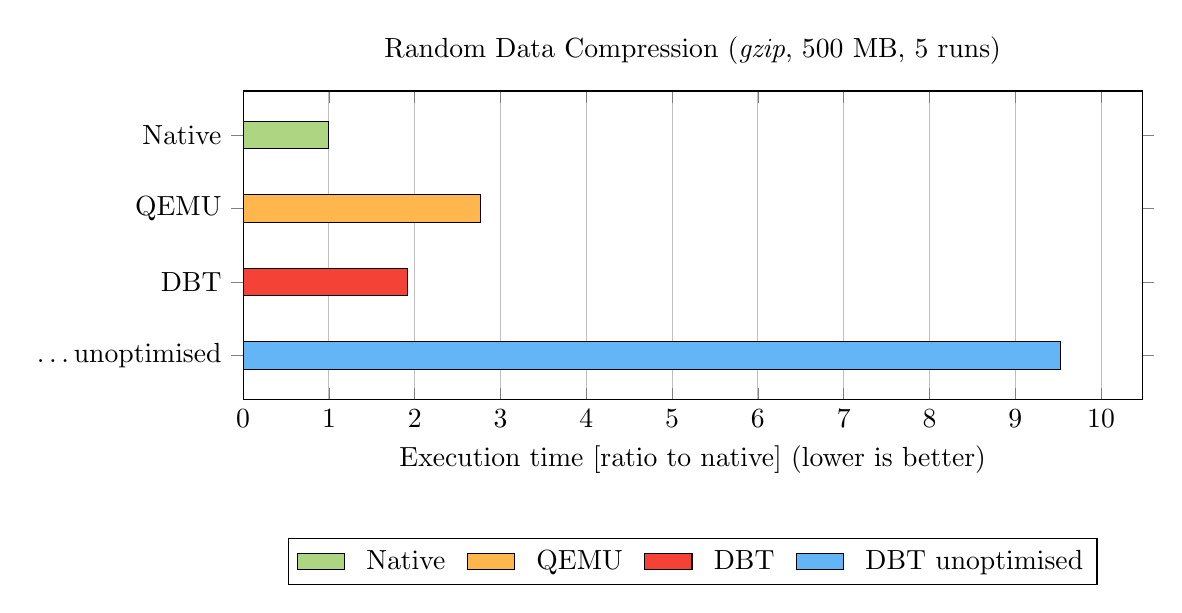
\begin{tikzpicture}
		\begin{axis}[%
			title = {Random Data Compression (\textit{gzip}, 500 MB, 5 runs)},
			xbar,
			area legend,
			xlabel = {Execution time [ratio to native] (lower is better)},
			symbolic y coords = {Native,QEMU,DBT,\ldots unoptimised},
			xmin = 0,
			bar shift = 0.0cm,
			y dir = reverse,
			enlarge y limits = {value=0.2, auto},
			xmajorgrids = true,
			height = 5.5cm,
			width = 13.0cm,
			legend style = {
				at = {(0.5, -0.45)},
				anchor = north,
				legend columns = 4,
				column sep = 0.2cm
			}
		]
			\addplot+ [
				fill=era-native,
				draw=black
			] coordinates {
				(1.0,Native) % 44.15
			};

			\addplot+ [
				fill=era-qemu,
				draw=black
			] coordinates {
				(2.767157418,QEMU) % 122.17
			};
			
			\addplot+ [
				fill=era-dbt-1,
				draw=black
			] coordinates {
				(1.911438279,DBT) % 84.39
			};
			
			\addplot+ [
				fill=era-dbt-2,
				draw=black
			] coordinates {
				(9.527180068,\ldots unoptimised) % 420.625
			};
			
			\legend{Native, QEMU, DBT, DBT unoptimised}
		\end{axis}
	\end{tikzpicture}
	\caption[Execution time of gzip compression]%
	{Execution time of gzip file compression (500 MB of random data, 5 runs) in seconds (normalised, lower is better).\\Unoptimised run executed with \texttt{----optimize=none}.}
	\label{fig:gzip-execution-time}
\end{figure}
% ===================================

Figure~\vref{fig:gzip-execution-time} lists the execution times of \textit{gzip} compressing a pseudo-random $500$ MB file sourced from \texttt{/dev/urandom}\footnote{Reproducible via \texttt{base64 /dev/urandom | head -c 524288000 > random.txt;}}.

Through our very efficient return address stack, recursive jump target translation, macro operation fusion and, most importantly, block chaining we are able to significantly outperform QEMU in random data compression by nearly 45\,\%.
The achieved performance of approximately two times the execution time of a native run is in line with the \textit{SPEC CPU 2017} results shown in figure~\ref{fig:spec-results}.

As mentioned in the caption, the unoptimised run was performed with the command line option \texttt{----optimize=none}, which disables all of the optimisation features mentioned above.
The translator will then have to translate every block one-by-one, jump back into the main loop on every block end and fetch the next position based on the current program counter.
























\section{Summary}
\label{sec:Summary}
Looking at the motivation the goal of outperforming QEMU~\cite{bellard2005qemu} is achieved consistently by "insert Project name here".
The performance is measured by~\textit{SPEC CPU 2017}~\cite{spec-cpu-2017} an industry-standardized, CPU intensive package of benchmark suites for measuring and comparing compute-intensive performance.
In most cases we can achieve a speed of around twice the native speed, but the tests also show areas for further optimization.
The quite significant performance increases in comparison to QEMU can be rooted to the specialisation in RISC--V to x86--64 translation lead to a straight forward design of the translation process and enabled specific optimizations for this guest-host pairing.

The benchmarks suits did not only help to ensure the performance of fish but equally important they tested the implementation in various scenarios and helped to discover bugs due to their assertion of the test programs' outputs.
Furthermore many unit tests were designed to assure the correct translation of (almost) every RISC--V instruction in diverse contexts.
All in all nearly 30.000 test cases are being executed by our own test suits based on~\textit{Googletest}~\cite{gtest} covering the RISC--V parser as well as the emitted x86--64 assembly.

Fish was focused on supporting and optimizing the core instruction set and integer extensions so far.
Support for floating point extensions however is already implemented and tested and will be benchmarked by~\textit{SPEC CPU 2017} as soon as possible.
Our preliminary tests nonetheless already show a huge performance increase in comparison with QEMU as a consequence of QEMU's emulation and fish's use of the native SSE--extension for floating point arithmetic.


Currently fish supports all base instruction sets and extensions needed for executing single threaded programs besides the \textit{"Q" Standard Extension}.
Future standard extensions such as the \textit{"B" Standard Extension} for bit manipulation can simple be added to fish when they come available by adding their opcode parsing to the parser and writing tailored translator functions.
Support of multithreading would be a bigger undertaking as it requires a redesign of fish's core to support the necessary memory consistency and atomicity of some memory access (\textit{"A" Standard Extension}).
Thus, this is not planned to be added in the near future.

Furthermore some operating system related features are not provided yet.
Specifically only a subset of the existing system calls is implemented and loading of dynamically linked libraries at runtime is not supported.

The next steps for generally improving fish would be implementing techniques used for integer arithmetic (e.g.\ lazy register replacement) for floating point arithmetic as well and supporting even more system calls.
Besides one could invest into on of the aforementioned areas specifically, for example applying a more rigid memory consistency model.

Concerning the performance optimization most time has been invested in the emitted code and reduction of context switches.
Benchmarking and optimization of the parsing and translation time has mostly been left out so far and might be due to optimization.


The current version of fish is capable of outperforming QEMU whilst providing almost the same functionality.
In some aspects e.g.\ floating-point arithmetic we are even ahead of QEMU by using the SSE-extension instead of emulating.
Also there is still potential for improvement the~\textit{SPEC CPU 2017} benchmarks demonstrate its usability in translating general purpose programs from RISC--V to x86--64.

\newpage
\section*{Appendices}
\begin{appendices}
\renewcommand\thesubsection{\Alph{subsection}}
\section{Download and installation instructions}
The source code for the translator can be downloaded by checking out the project's git repository.
Take care to either \texttt{git clone} the repository with the option flag \texttt{--recursive}, or to run the command
\begin{lstlisting}
	git submodule update --init
\end{lstlisting}
as the repository contains submodules that are required for compilation.

Then, the translator can be built by exeucting
\begin{lstlisting}
	sudo apt-get -y install gcc g++ cmake make autoconf meson
	mkdir build && cd build && cmake .. && make
\end{lstlisting}
in the root directory of the repository.
Note that the build requires CMake version 3.16 or above.
This will build two artifacts:
\begin{description}
	\item[translator] The actual dynamic binary translator.
	For details on the usage, see the section below, or execute \texttt{./translator -h}.
	
	\item[test] The unit test binary.
	It can be executed via \texttt{./test} and performs extensive unit testing of the RISC-V instruction implementations, the cache, register file, as well as the parser.
\end{description}

\section{Executable program requirements}
We can execute binaries compiled via the tools provided in the RISC-V GNU toolchain\footnote{For further information as well as download and usage instructions, see \url{https://github.com/riscv/riscv-gnu-toolchain} (last accessed on 25.09.2020).}.
The executables need to be linked statically (pass the flag \texttt{-static} to gcc when compiling), as the translator does not support dynamically linked files.

% todo update if floating point comes into play
We currently support binaries compiled for the architecture specifier \texttt{rv64ima}, meaning the compiler is free to utilise the base integer instruction set (\texttt{i}), as well as the instructions provided by the multiplication (\texttt{m}) and atomic standard extensions (\texttt{a}).
This can be achieved by passing \texttt{-march=rv64ima} to gcc\footnote{Note that some architecture strings require recompilation of the toolchain. Also, the aforementioned option implies \texttt{-mabi=lp64}.}.

\section{Using the translator}
% this assumes the state of opt_rewrite, todo update as necessary
\begin{lstlisting}
	./translator [translator option(s)] -f <filename> [guest options]
\end{lstlisting}

Seen above is the syntax for executing the translator with a guest program.
All possible translator options are described in the help text, as seen by executing \texttt{./translator -h}.
Every option after the filename specified via the \texttt{-f} flag is passed along to the guest in its \texttt{argv}, so all options intended for the translator must be passed before \texttt{-f}.

The command line options also include the ability to analyse (\texttt{-a}) the binary to produce a detailed breakdown of which instruction mnemonics and registers the guest will use when executed.
Furthermore, it includes the ability to time the execution of only the guest program by passing the flag \texttt{-b}.

Logging can be controlled by passing the requested category to the \texttt{----log} flag as detailed in the help, and can provide insights into the state of the translator during execution or debugging.
Lastly, it is also possible to selectively disarm optimisation features like the return address stack, block chaining or recursive jump target translation via \texttt{----optimize}.















\end{appendices}

\newpage
\listoftables
\listoffigures

\newpage
\bibliographystyle{ieeetr}
%\addcontentsline{toc}{section}{References}
\bibliography{paper}
\end{document}
